\documentclass[tikz,border=6pt]{standalone}
\usepackage[T1]{fontenc}
\usepackage{lmodern}
\usepackage{amssymb}
\usetikzlibrary{positioning,arrows.meta,calc}

\newcommand{\ltb}{$<^{\mathrm{b}}$}

\begin{document}
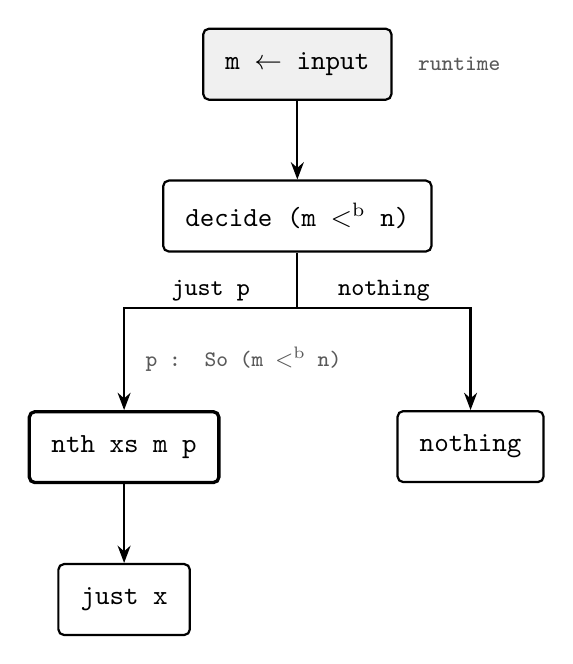
\begin{tikzpicture}[
    >={Stealth[length=2.2mm]},
    box/.style={draw, thick, rounded corners=2pt, minimum height=9mm,
                inner xsep=8pt, font=\ttfamily},
    io/.style={box, fill=gray!12},
    ok/.style={box, very thick},
    edgelbl/.style={font=\ttfamily\small, inner sep=2pt},
    note/.style={font=\ttfamily\footnotesize, text=gray!70!black},
  ]
  \node[io]                   (m)   {m $\leftarrow$ input};
  \node[box, below=10mm of m] (dec) {decide (m \ltb{} n)};

  \coordinate (fork) at ($(dec.south)+(0,-7mm)$);

  \node[ok,  anchor=north] (nth)  at ($(fork)+(-22mm,-13mm)$) {nth xs m p};
  \node[box, below=10mm of nth]                               (just) {just x};
  \node[box, anchor=north] (none) at ($(fork)+( 22mm,-13mm)$) {nothing};

  \draw[->, thick] (m) -- (dec);
  \draw[thick] (dec) -- (fork);
  \draw[->, thick] (fork) -| node[edgelbl, above, pos=0.25] {just p}  (nth);
  \draw[->, thick] (fork) -| node[edgelbl, above, pos=0.25] {nothing} (none);
  \draw[->, thick] (nth) -- (just);

  \node[note, anchor=west] at ($(nth.north)+(1.5mm,6.5mm)$) {p : So (m \ltb{} n)};
  \node[note, right=2mm of m] {runtime};
\end{tikzpicture}
\end{document}
